\section{Related works: Evolutionary Game Theory on Graphs}
Evolutionary game theory on graphs is relevant because populations interact only
with a fixed subset of neighbors, which has been proposed as a mechanism for the
emergence of cooperation among unrelated individuals
\cite{cardillo2010coevolution}.  
In this framework, each agent is characterized by a strategy and an update rule.
For example, in the weak Prisoner’s Dilemma, strategies are Cooperation (C) or
Defection (D), while update rules include replicator (REP), Moran-like (MOR),
or unconditional imitation (UI).  
Cardillo et al.~\cite{cardillo2010coevolution} studied the co-evolution of
strategies and update rules on adaptive networks.  
A different example is the Ultimatum Game \cite{sinatra2009ultimatum}, where
strategies evolve depending on past payoffs and the network structure influences
the spread of fair or egoistic behavior.  
This setting highlights the role of altruistic acts (costly to the individual
but beneficial to others) as a key mechanism for cooperation.

\section{Empirical Network (Karate Club)}

\noindent\textbf{Basic features.}  
Nodes: $n=34$, edges: $m=78$, undirected and unweighted.  
Degrees range from $1$ (peripheral members) to $17$ (instructor hub).  
Average degree $\bar{k}\approx 4.6$, clustering coefficient $\approx 0.57$, and
average path length $\approx 2.4$ (diameter $=5$).  
The network naturally splits into two groups (instructor vs president),
frequently used as a benchmark for community detection. \cite{zachary1977karate}

\begin{figure}[H]
\centering
    \begin{minipage}[t]{0.48\textwidth}
        \centering
        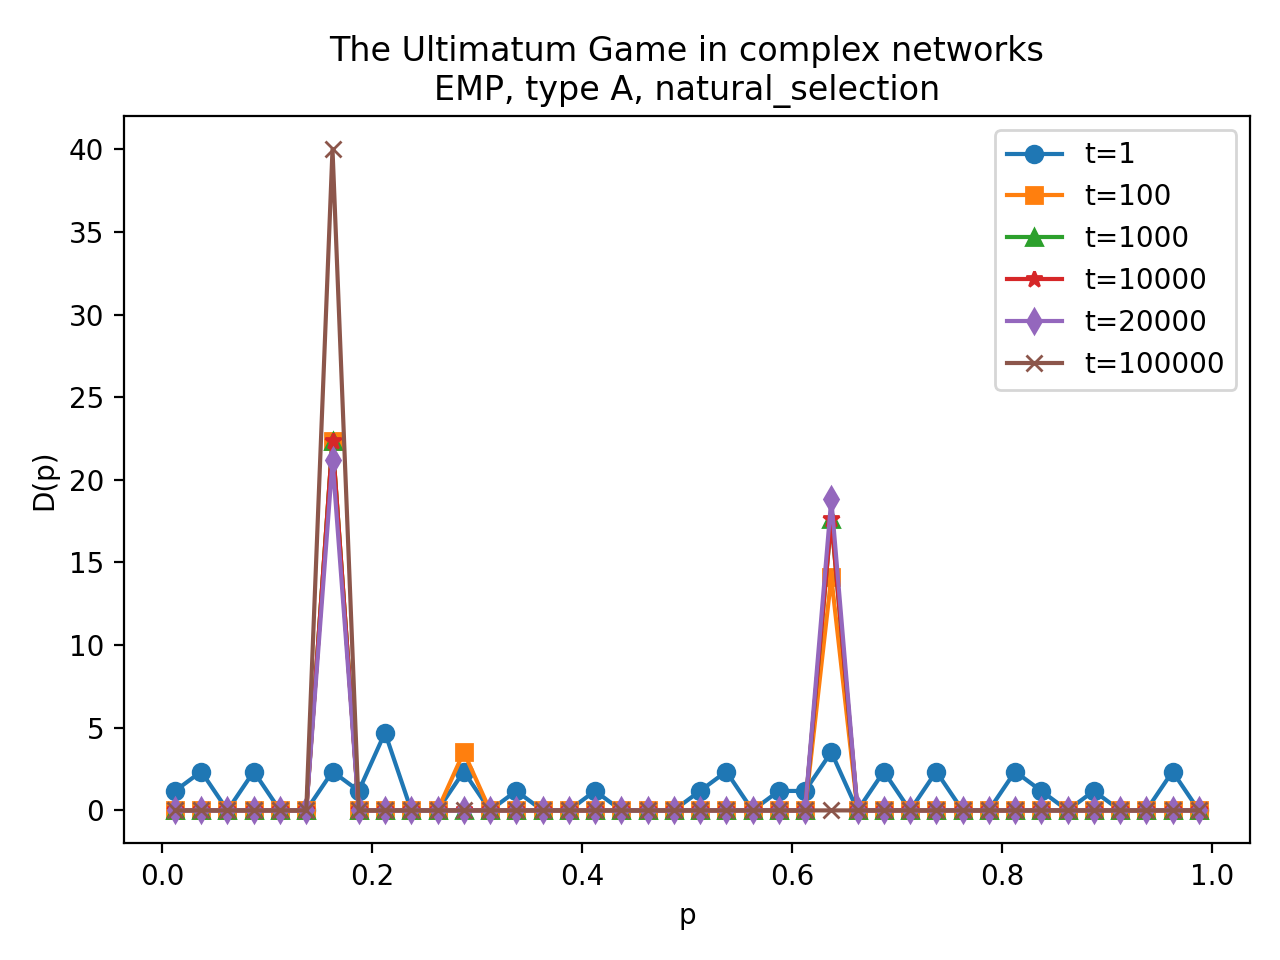
\includegraphics[width=\textwidth]{images/TASK1/Dp_EMP_A_natural_selection.png}
        \captionof{figure}{Proposal distribution $D(p)$ in EMP network with A players under natural selection.}
        \label{fig:EMP_Dp_A_NS}
    \end{minipage}
    \hfill
    \begin{minipage}[t]{0.48\textwidth}
        \centering
        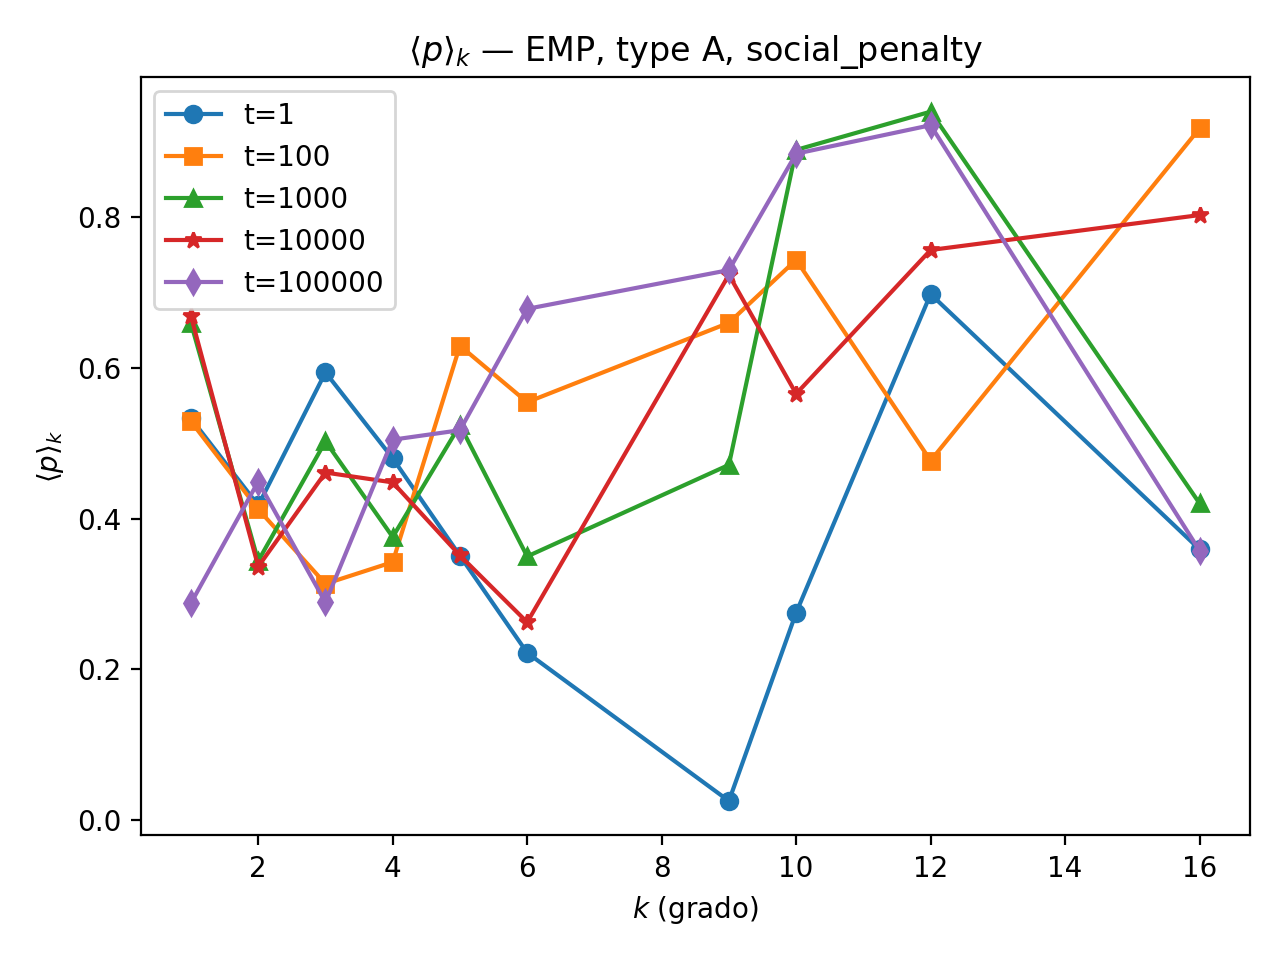
\includegraphics[width=\textwidth]{images/TASK1/p_by_degree_EMP_A_social_penalty.png}
        \captionof{figure}{Average proposal $\langle p \rangle$ by degree class in EMP network under social penalty.}
        \label{fig:EMP_p_by_degree_A_SP}
    \end{minipage}
\end{figure}

\noindent In Figure~\ref{fig:EMP_Dp_A_NS}, proposals show two clear peaks (intermediate
and high $p$), reflecting the heterogeneity of the empirical network.  
When strategies are analyzed by degree (Figure~\ref{fig:EMP_p_by_degree_A_SP}),
high-degree nodes tend to propose more. This suggests that under social penalty
they are pressured into fairer behavior, since their removal would have a strong
impact on the system.

\section{Other simulations}

\begin{figure*}[h!]
    \centering
    \setlength{\tabcolsep}{2pt}
    \begin{minipage}[t]{0.48\textwidth}
        \centering
        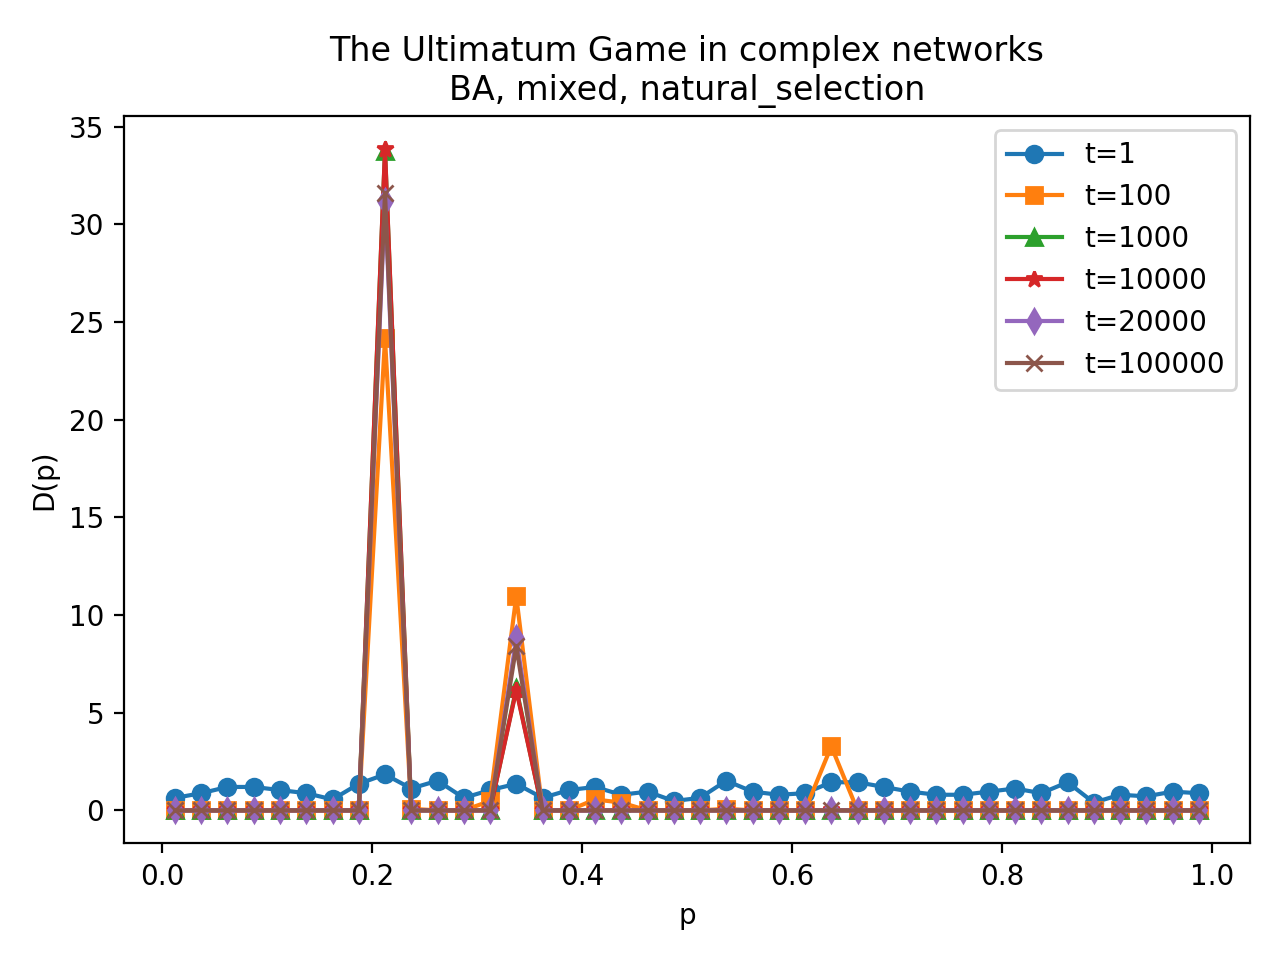
\includegraphics[width=\textwidth]{images/TASK1/Dp_BA_MIX_natural_selection.png}
        \subcaption{Proposals $D(p)$ with mixed players (A,B,C) in BA network.}
        \label{fig:Mix_Dp}
    \end{minipage}
    \hfill
    \begin{minipage}[t]{0.48\textwidth}
        \centering
        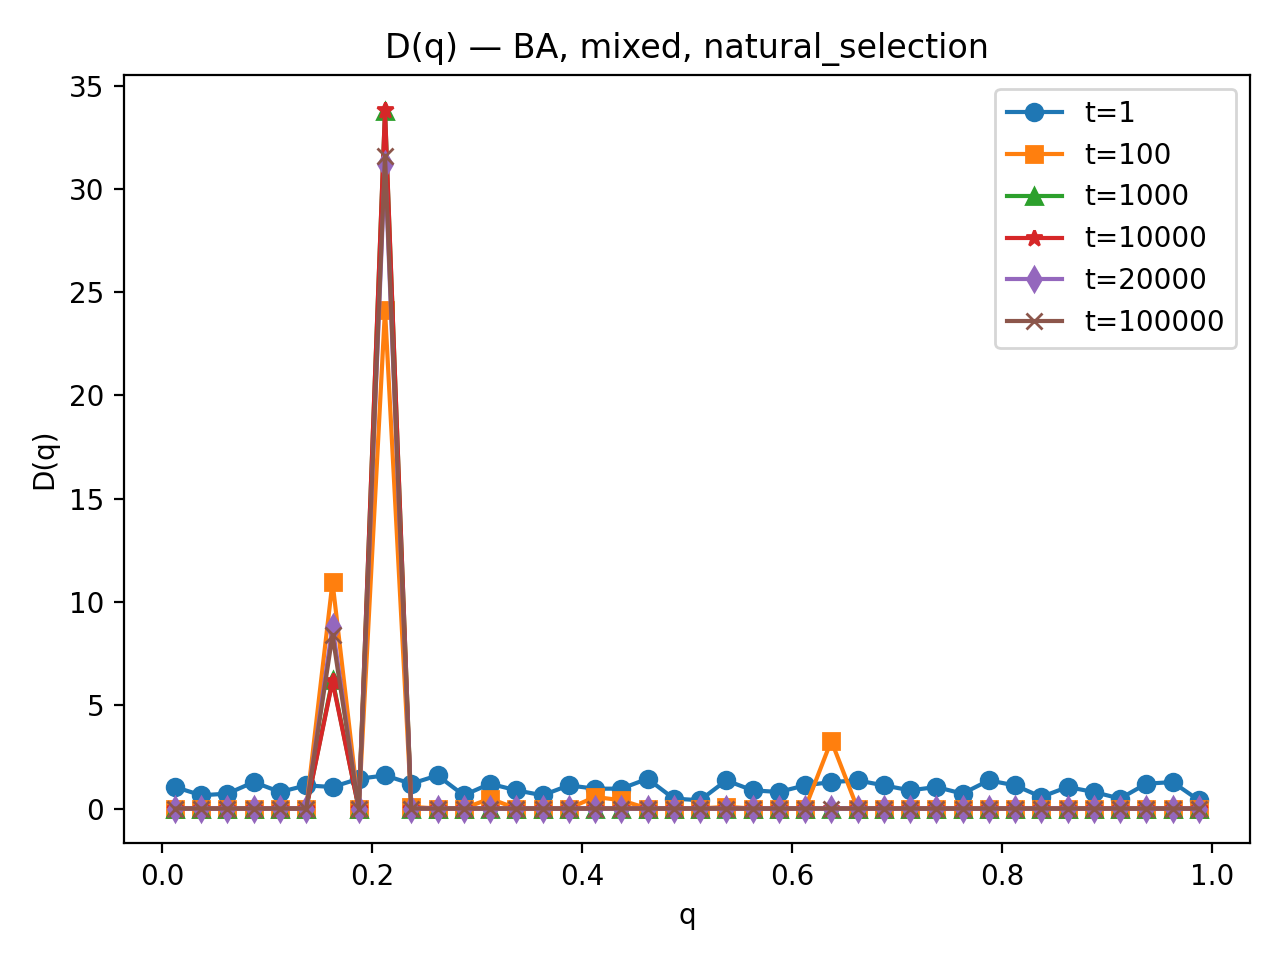
\includegraphics[width=\textwidth]{images/TASK1/Dq_BA_MIX_natural_selection.png}
        \subcaption{Acceptances $D(q)$ with mixed players (A,B,C) in BA network.}
        \label{fig:Mix_Dq}
    \end{minipage}
    \caption{BA network with a mixed population of A, B, and C players under natural selection.}
    \label{fig:BA_Mix}
\end{figure*}

\noindent In the BA network with mixed player types (Figure~\ref{fig:BA_Mix}), proposals
$D(p)$ become multi-modal (Fig.~\ref{fig:Mix_Dp}) and acceptance thresholds
$D(q)$ show several persistent peaks (Fig.~\ref{fig:Mix_Dq}).  
This indicates that heterogeneous strategies can coexist: fair, pragmatic, and
random behaviors interact, generating diversity both in offers and in
acceptances.  
Compared to homogeneous populations, the presence of multiple player types
prevents convergence to a single equilibrium and sustains residual variability.



\noindent The heatmap in Figure~\ref{fig:ER_heatmap_pq} shows the joint distribution of
offers $p$ and thresholds $q$ in the ER network with C players under social
penalty at $t=100000$.  
The highest density lies in the lower-right region (high $p$, low $q$), meaning
that most players converge to offering generous proposals while at the same time
accepting almost any amount.  
This reflects the effect of the social penalty: nodes are pressured to avoid the
lowest payoff, which drives proposers towards fairness and responders towards
opportunism.  
Additional scattered clusters at intermediate values of $p$ and $q$ reveal
alternative equilibria, but the dominant attractor corresponds to this
“asymmetric cooperative” regime.  
The joint representation is therefore crucial, as it shows that fairness (high
$p$) and tolerance (low $q$) emerge together, a pattern hidden in separate
distributions of $p$ and $q$.

\begin{figure}[H]
    \centering
    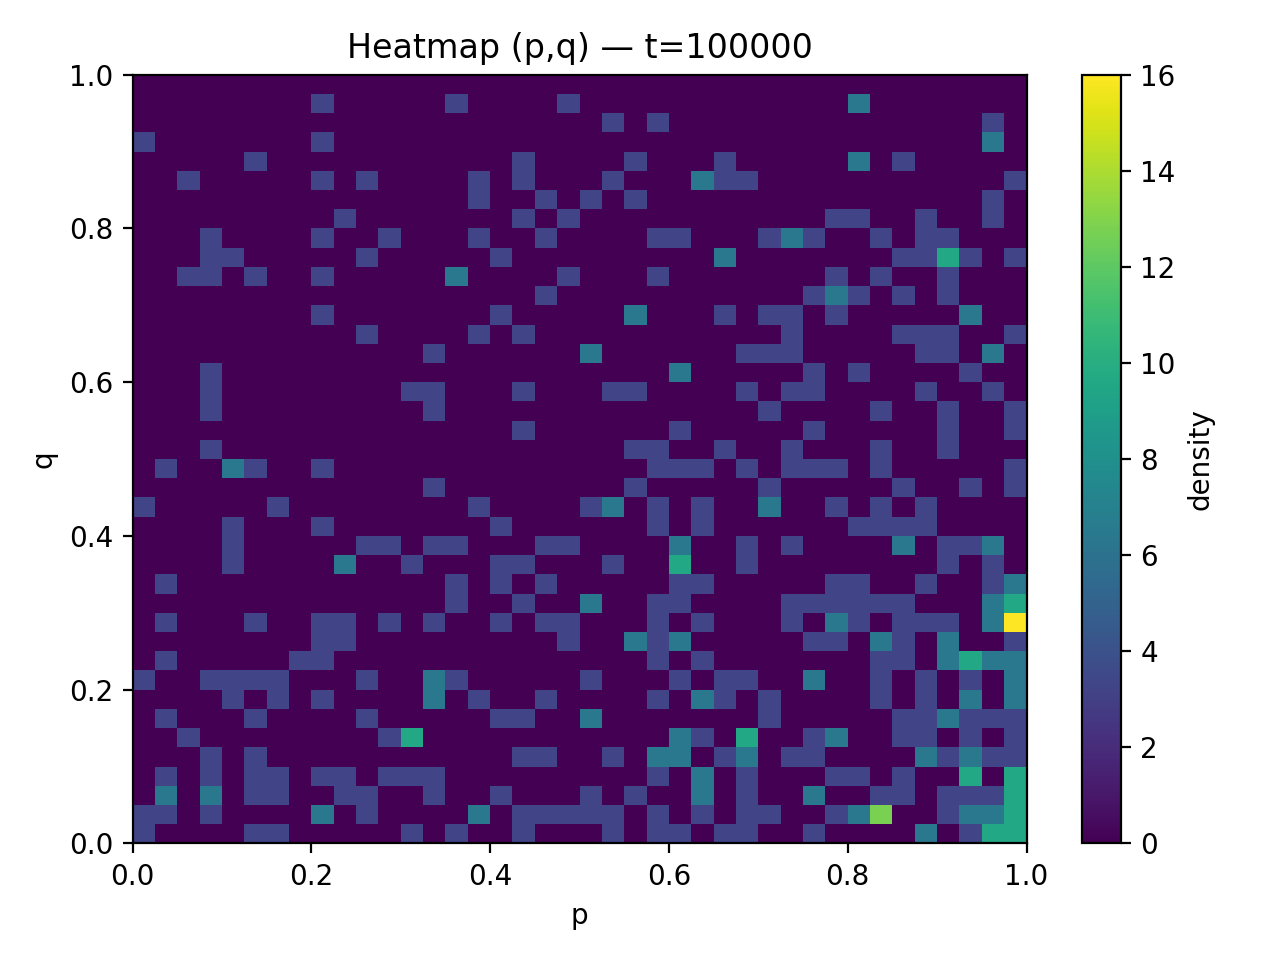
\includegraphics[width=0.75\linewidth]{images/TASK1/heatmap_pq_t100000_ER_C_social_penalty.png}
    \caption{Heatmap of joint distribution $D(p,q)$ in ER network with C players under social penalty ($t=100000$).}
    \label{fig:ER_heatmap_pq}
\end{figure}


\subsection*{Summary of additional results}
The additional simulations confirm the trends observed in the main text:
\begin{itemize}
    \item Empirical networks show bimodality and degree effects, with hubs driven
    to fairer strategies under social penalty.
    \item BA networks with mixed player types (A, B, C together) preserve strong
    heterogeneity: fair, pragmatic, and random strategies coexist, leading to
    multimodal distributions in both $p$ and $q$.
    \item Heatmaps of $(p,q)$ reveal that the dominant equilibrium corresponds to
    high offers ($p$ large) and low acceptance thresholds ($q$ small). This
    asymmetric cooperative regime is sustained by the social penalty mechanism
    and is not visible from marginal distributions alone.
\end{itemize}
Overall, these supplementary cases reinforce the idea that network structure,
player diversity, and update dynamics jointly determine how cooperation and
fairness spread in populations.


